\documentclass[12pt]{article}
\usepackage[slovene]{babel}
\usepackage[utf8]{inputenc}
\usepackage{makeidx}
\usepackage{pifont}
\usepackage{listings}  
\usepackage{hyperref}  
\usepackage{graphicx}
\usepackage[margin=0.8in]{geometry}
\usepackage[xindy,toc,acronym]{glossaries}

\let\stdsection\section
\renewcommand\section{\newpage\stdsection}

\title{Sistemi za detekcijo napadov}
\author{Domen Kožar, Andraž Brodnik}
\begin{document}

\maketitle

\tableofcontents

\section{Povzetek}
Teoretični del zajema razlago sistemov za detekcijo napadov (IDS) in preprečevanje napadov (IPS) 
ter njihove podskupine. 
Osredotočili se bomo na sisteme, ki opazujejo promet na omrežnem vmesniku (NIDS/NIPS).
\\*
\\*
V praktičnem delu pa smo namestili in nastavili sistem Snort.

\section{Uvod}

Namen seminarske naloge se je seznaniti s sistemi za zaznavanje vdorov ter s sistemi za preprečevanje vdorov. 
Kako sestaviti osnovno politiko (policy) za tak sistem, kakšne napade lahko detektiramo, ter priporočljive obrambne mehanizme.
\\*
\\*
Dandanes se srečujemo z novicami o nepoblaščenih vdorih v informacijske sisteme.
Takšni vdori lahko uničijo podjetje ali zasebnost uporabnikov,
kar pomeni, da je racionalno investirati nekaj tehničnih ur v postavitev sistema, ki bi lahko (ni pa nujno) taksen vdor preprečil ali pa zaznal poskus vdora.
To nam koristi, da vidimo na kaksen način je napadalec napadel naš sistem, ter kaj je storil. 
\\*
\\*
Kljub temu, da je naša varnostna politika v skladu z dobro prakso (menjava gesel, dvonivojska avtentikacija, požarni zidovi,
varne aplikacije, tuneliranje prometa, up-to-date strežniki), ne smemo biti preveč zadovoljni s sami sabo ter moramo postavit tudi sistem za detekcijo in/ali preprečevanje napadov.
\\*
\\*
Naj bralca opozorimo tudi na dejstvo, da `nepravilno' konfiguriran IDS ali IPS sistemi lahko globoko posežejo
tudi v zasebnost posameznika, kar ni v skladu z ustavo Republike Slovenije in drugimi pravnimi akti.
IDS in IPS sistemi se lahko uporabljajo tudi kot DPI (deep packet inspection) sistemi, kar pomeni, da ne gledamo
samo glav paketnih protokolov ampak tudi aplikacijski nivo (aplikacijski protokol oz.\ vsebino), 
zato nastavljajmo IDS in IPS sisteme odgovorno, podatke pa shranjujmo z največjo skrbjo.

\section{Teoretični del}



\subsubsection{IDS} % (fold)
\label{ssub:IDS}


Sistemi za detekcijo napadov (intrusion detection system), krajše IDS
so sistemi, katera naloga je analizirati podatke na omrežju ali sistemu samem
ter zaznati poskuse vdora ali pa vdor sam.
\\*
Naj omenimo, da so tej sistemi namenjeni ponudnikom storitev (podjetjem, inštitucijam, posameznikom)
v večini niso namenjeni omrežnim operaterjem, razen če želimo preprečevati napade na naše omrežne elemente. 
Ne moremo pa vsiljevati pravil za vse naše uporabnike. Včasih pa je bilo tega prometa za analizo preveč, a vendar
so se časi spremenili in to ni več glavna omejitev.
\\*
Delimo jih na dve glavni skupini:

\begin{itemize}
    \item NIDS (network intrusion detection system)
    \item HIDS (host intrusion detection system)
\end{itemize}

% subsubsection IDS (end)


\subsection{NIDS}

Sistemi, katerim je glavni vir podatkov za analizo izključno omrežje se imenujejo NIDS sistemi (network intrusion detection system).
Kar pomeni, da opazujejo ves dohodni in izhodni promet, nato pa indentificira sumljive vzorce, ki bi lahko kazali na napad na omrežje ali nek sistem.
\\*
Bralcu bo po vsej verjetnosti poznan program WireShark ali pa tcpdump.
NIDS ponavadi delujejo podobno kot zgoraj omenjena programa. Program zajema vse paketke, ki jih vidi na omrežnem vmesniku,
nato jih premerja s pravili v svoji bazi, sumljive pakete ali niz paketov pa zabeleži ali pa si ustrezno napiše informacije o njih.

\subsubsection{Komponente} % (fold)

\begin{figure}[htb]
\begin{center}
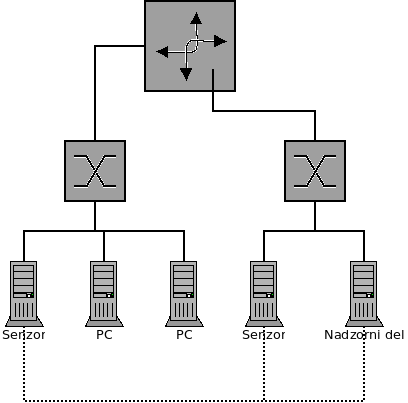
\includegraphics[scale=0.5]{komponente.png}
\end{center}
\caption{Primer postavitev komponent}
\label{komponente}
\end{figure}

Sami NIDS sistemi so ponavadi razdeljeni na 2 dela:
\begin{itemize}
    \item Senzor
    \item Nadzorni del
\end{itemize}

Senzorji so programi, ki zajemajo paketke na določenem delu omrežja jih analizirajo nato pa pošljejo nadzornem delu.
\\*
Takšna delitev ima več prednosti. Prva prednost je, da se dogodki/alarmi počiljajo naprej torej so reproducirani, tako je praktišno nemogoce za napadom pobrisati sledi.
Hkrati lahko zajemamo več omrežjij, ki so na različnih lokacijah brez, da bi promet preosmerili na centralno lokacijo.
Oz.\ lahko dvignemo več instanc (slovenski prevod primerek je neprimeren) senzorjev na enem samem strežniku, kar nam omogoča bolšo uporabo računskih virov na strežniku.
To nam seveda oteži samo nastavitev (konfiguracijo) sistema, kar pomeni, da je takšna postavitev smiselna za večja podjetja.

%  Komponente (end)

\subsubsection{Detekcija napadov} % (fold)

Kako poteka sama detekcija napadov? 
NIDS sistemi imajo vgrajeno bazo odtisov napadov. Če je dogajanje na mreži podobno, opisanem napadu v bazi
bo NIDS sistem to napisal v dnevnik ali pa si celo shranil napad (v pcap datoteki). 
NIDS sistemi so sumljičavi, glede velikosti, samega protokola in količine paketov.
NIDS sistemi imajo vgrajene tudi logične avtomate, torej se zavedajo tudi paketov pred nekim paketom in po njem.

%  Detekcija napadov (end)

\subsubsection{Lokacija v omrežju} % (fold)

\begin{figure}[htb]
\begin{center}
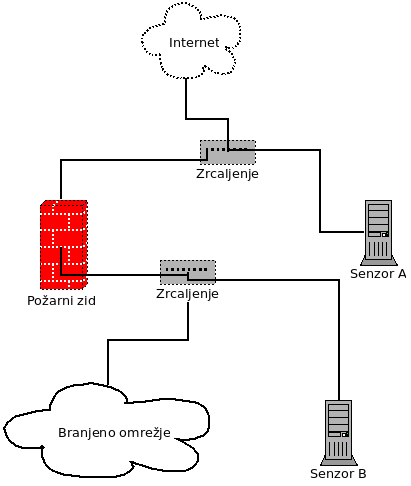
\includegraphics[scale=0.5]{pozicija.png}
\end{center}
\caption{Primer dveh lokacij senzorjev: Senzor A pred požarnim zidom in senzor B za njim}
\label{pozicija}
\end{figure}

NIDS sisteme lahko postavimo na več delov v sistemu. Najbolj pogosto je za požarnim zidom.
Z tem zajemamo vse pakete, ki jih požarni zid ni zavrgel. To nam sicer ne, da celotnega uplogleda v vse napade.
Nam pa zmanjša količino podatkov, ki jih moramo obdelati. Napadi, ki nam ne pridejo skozi požarni zid načeloma niso nevarni.
\\*
NIDS senzorje imamo lahko razdeljene tudi na različnih fizicnih lokacijah ali logicnih lokacijah, ker ni mogoče vse realizirati z enim senzorjem ali pa si to ne želimo (zahtevana je separacija).

% Lokacija v omrezju (end)

\subsubsection{Omejitve NIDS} % (fold)

\paragraph{Lažni alarmi} % (fold)
Pomembna mejitev je pogostost lažnih alarmov.
Noben NIDS sLažni alarmiistem ne more preprečit pojavljanje lažnih alarmov.
V večino NIDS sistemom je mogoče dodati tudi vzorce lažnih alarmov. 
V bazo dodamo vzorec, ki nam sproži alarm vendar NIDS sistem najde pravilo, da je to lažni alarm.
% paragraph lažni alarmi (end)

\paragraph{TCP tok/IP fregmentacija} % (fold)

Sestavljanje TCP toka podatkov (stream)/Sestavljanje IP paketkov (zaradi defregmentacije)
\\*
Kot omenjeno kdaj analiziramo celotne TCP toke podatkov, da lahko zaznamo nevarnost. To pomeni, da moramo shranjevati paketke. 
Pri napadih mnogokrat ne zaklučimo toka podatkov, kar pomeni, da se more pri shranjevanju tokov podatkov NIDS obnasati zelo specifično. Podobne probleme imamo tudi pri IP paketih. 
Kot vemo imamo omejen polnilnik. Predstavljate si lahko koliko paketkov lahko shranimo na 10Gbit/s vmesniku.
% paragraph TCP tok/IP fregmentacija (end)

%  Omejitve NIDS (end)

\subsubsection{Stvari, ki jih moramo premisliti} % (fold)

\paragraph{Operacijski sistem} % (fold)

Pomemben je operaciski sistem. Ponavadi jo NIDS sistemi navoljo za vse sisteme,
tako Windows NT kot Unix ter ostale. Neki sistemi lahko tečejo na več različnih, tako ni nič nenavadnega
da imamo senzor na OpenBSD, managment pa na Windows NT sistemu.
Pomembno je da sistemski administratorji poznajo platformo na kateri teče NIDS ali del njega, saj je pomembno, da je ta ustrezno zasčitena.

% paragraph Operacijski sistem (end)

\paragraph{Podprti omrezni vmesniki} % (fold)

Pomembno je da se zavedamo, da niso podprti vsi omrežni vmesniki. Vecina sistemov podpira samo ethernet vmesnike.

% paragraph Podprti omrezni vmesniki (end)

\paragraph{Alarmi} % (fold)

Pomembno je, da se odločimo kakšne načine obveščanja se bomo poslužili. Ponavadi so detekcije (alarmi) razdeljeni v različne tipe ali nivoje.
Glede na katere določimo kanal obveščanja. 
Nekatere napade lahko zgolj napišemo v dnevnik, za nekatere pošljemo e-posto skrbniku ali operatorju v nekaterih primerih pa pošljemo SMS.

% paragraph Alarmi (end)

\paragraph{Pisanje dnevnikov in poročil} % (fold)

Vsi NIDS sistemi pišejo alarme v dnevnike, torej lahko za nazaj pogledamo, kaj se je dogajalo. Določeni sistemi pa omogočajo tudi pošiljanje avtomatsko generiranih porocil (npr.\ dnevnih).
% paragraph Pisanje dnevnikov in porocil (end)

\paragraph{Vzdrževanje} % (fold)

Pomemben segment je tudi vzdrževanje. Vprašanja glede tega so. Ali sem nam baza odtisov, sama posodablja ali pa jo moramo avtomatsko posodobiti? Kako se posodablja jedro? Moramo za posodobitve baze plačevati. Koliko stane licenca?
Imamo več alternativnih virov odtisov? Je okoli odtisov v bazi zbrana skupnost ali pa celo akademsko okolje.
Koliko fleksibilni so ti mehanizmi. Koliko pogosto moramo posadabljati. 
Stvar zavisi od naših izkušenj in od izbranega sistema. Ni pa enoličnega odgovora za takšna vprašanja.
% paragraph Vzdrzevanje (end)


\paragraph{Izgled nadzornega sistema} % (fold)

Pomemben je izgled nazornega dela. Ali je nadzorni del prijazen in ga hitro razumemo.
Nadzorni deli niso namenjeni konfiguraciji, ampak predvsem prikazu alarmov, a lahko kjub temu omogočajo preproste nastavitve.
Vecina komercialnih sistemov nam ponuja grafične vmesnike. Realizirane za različne platforme ali pa kar spletni vmesnik.
Določeni sistemi nam dajo na razpolago programerski vmesnik (API), nato pa vzamemo drug projekt za prikaz rezultatov.

% paragraph Izgled nadzornega sistema (end)


\paragraph{Skalabilnost} % (fold)

Skalabilnost je pomemben aspekt, če nacrtujemo sistem za omrežja, ki so velika ali pa se bodo razširila. 
V tej točki, nas zanima ali NIDS sistem izkorišča vse procesorje na strežniku oz.\ kako to doseči ali lahko paktetke pošiljamo naprej. Drugim računalnikom in tako dosežemo neko kolektivno intelegenco.
Koliko paketkov lahko realno zajamemo in obdelamo, preden jih začnemo spuščati (ne analizirati).
% paragraph Skalabilnost (end)

%  Stvari, ki jih moramo premisliti (end)

\subsection{NIPS}

Veliko smo napisali o NIDS sistemih, vendar kaj so NIPS (network intrusion prevention system) sistemi?
NIPS je sistem za preprečevanje napadov, ki glede na alarme NIDS vgrajenega sistema izvedejo določene akcije, ki ta napad preprečijo ali pa ga ustavijo.

Bralca naj te termini ne zmedejo saj se jih ne uporablja strikno. Korak od IDS do IPS sistema je zelo majhen zato se veliko IDS sistemov deklarira kot IPS.

\subsubsection{Načini preprečevanja} % (fold)

\paragraph{Spreminjanje pravil v požarnem zidu} % (fold)

Najbolj pogosto NIPS sistemi spreminjajo pravila požarnega zidu.
Če je NIPS sistem vgrajen v požarni zid potem je to sila preprosto.
Drugače pa mora komunicirati preko malih programov ali pa protokolov za oddaljen nadzor (SSH, netrpc).

Kot primer si predstavljamo, da NIPS sistem zazna napad napise pravilo v požarni zid, da vse pakete, ki prihajajo iz izvornega IP naslova napadalca zavrze za določeno časovno obdobje (npr. 20 minut).

Poslužimo se lahko seveda tudi filtriranje glede na TCP/UDP port.

Ta način se uporablja v večini primerov.

% paragraph Spreminjanje pravil v pozarnem zidu (end)

\paragraph{Spreminjanje usmerjanja} % (fold)

Če imamo možnost ali pa veliko prometa lahko uporabimo zgornji način malo drugače.
V primeru, da so napadi res hudi. Lahko usmerjevalni protokol nastavimo tako, da nastavimo neveljavno pot (null route) za napadalčev naslovni prostor.

% paragraph Spreminjanje usmerjanja (end)

\paragraph{Obveščanje/nadzor ostalih storitev} % (fold)

Možno je tudi pisanje posebnih pravil, ki začasno spremenijo nastavitve aplikacijskih strežnikov in drugo.

% paragraph Obveščanje ostalih storitev (end)

% subsubsection Nacini preprecevanja (end)

\subsubsection{NIDS/NIPS produkti} % (fold)

Tipične sistemi v praksi so:
\begin{itemize}
    \item Snort (odprtokodni sistem)
    \item Cisco IPS/IDS
    \item Niksun NetDetector
    \item ISS RealSecurea
\end{itemize}

Naj omenimo najbolj pogosta:


\paragraph{Snort} % (fold)
\label{par:Snort}

\begin{figure}[htb]
\begin{center}

\includegraphics[scale=0.8]{Snort_ids_logo.png}
\end{center}
\caption{Snort}
\label{snort_img}
\end{figure}

Snort\cite{snort} je odprtokodni NIDS/NIPS sistem, ki ga razvija podjetje Sourcefire\cite{sourcefire} z svojimi 560 zaposlenimi.
Prvotno je leta 1998 sistem Snort napisal Martin Roesch, ki je sedaj tehnični direktor podjetja. 
Snort je čez leta postajal čedalje bolj pomemben v informacijski industriji, uspeh pa je zgled za celotno odprtokodno skupnost.
\\*

Snort je izdan pod GPL licenco, napisan je v C programskem jeziku ter deluje na več operacijskih sistemih.
\\*

Snort ima močno komercialno podporo. Glavna njihova storitev je ponudba pravil za snort konfiguracijo.
\\*

Ponavadi ga namestimo na GNU/linux sistem. Pri tem je lahko strojna oprema poljubnih proizvajalcev, se pozna če imamo PCI-X režo za omrežni vmesnik.
Strežnik ima lahko več jeder za obdelavo podatkov. Snort je mogoče poganjati samo na enem jedru, vendar lahko procesi med sabo dobro komunicirajo (clustering), saj je snort narejen z mislijo obdelave veliko podatkov.
Za neko srednje podjetje se priporoča strežnik, ki ima dva omrežna vmesnika ter 4 jedra ali več.
\\*

Dva omrežna vmesnika sta nujna saj na enem zajemamo promet, na drugem shranjujemo paketke na NAS, izvajamo IPS akcije/sankcije ter nadzorujemo sistem. Taksnih postavitev smo navadno vajeni pri omrežnih elementih, kjer imamo za nadzor ločene komunikacijske kanale.
\\*

OISF\cite{oisf} je začel razvijati novo implementacijo, ki uporablja Snort pravila imenuje se Suricata.
Glavne prednost je da lahko uporaljablja več jeder ter privzeto podpira IPv6.

% paragraph Snort (end)

\paragraph{Cisco} % (fold)
\label{par:Cisco}


\begin{figure}[htb]
\begin{center}

\includegraphics[scale=0.7]{cisco_logo.png}
\end{center}
\caption{Cisco}
\label{cisco_img}
\end{figure}

Cisco ponuja te sisteme v ASA seriji 5000\cite{cisco5000}, kot je razvidno na njihovi strani.
Najbolj zmogljivi sistem lahko obdela 400Mbit/s podatkov, to pomeni z hkratnim delovanjem tako požarnega zidu, kot IPS sistema. 
\\*
Cisco ima stvari dobro integrirane med vsemi napravami. To omogoča njihov sistem SIO (Security Intelligence Operations). Hkrati pa nam osvežujejo pravila.

% paragraph Cisco (end)



% subsubsection NIDS produkti (end)

\subsection{HIDS}

HIDS sistemi (host intrusion detection system) so sistemi za detekcijo napadov, ki delujejo na samem strežniku ali pa napravi,
ki ponuja neko storitev odjemalcem.
Torej HIDS sistem zanima samo gostitelj (host).
Zaznava tudi paketke iz omrežja, vendar samo tiste, ki so namenjeni gostitelju.
Ne zaznava pa samo paketkov.
To pomeni da imamo senzorje na vsaki napravi, ki jo želimo ščititi.
Te senzorje ponavadi imenujemo agenti.
Zakaj bi postavili se HIDS na strateško pomembnih napravah?
Primarno, ker gre za drug nivo zaznave in preprečevanja. 

\subsubsection{Omejitve HIDS} % (fold)

Glavni problem HIDS sistemov je, da so tesno povezani z platformo na kateri delujejo 
oz.\ sam operacijski sistem.
Kot prej omenjeno moramo imeti na vsaki napravi nameščenega agenta. Ta agent ponavadi vedno pošilja vse podatke naprej nadzornemu sistemu.
Nikoli se ne zanašamo, da je sistem pod našim nadzorom in v njega se ni bilo vdrto.

% subsubsection Omejitve HIDS (end)

\subsubsection{Načini zaznav napadov} % (fold)

\paragraph{Poslušanje omrežnega vmesnika} % (fold)

HIDS tudi posluša omrežni vmesnik na napravi. 
Podobno kot to dela NIDS, kar smo opisovali v prejšnih poglavjih.

% paragraph Poslusanje omreznega vmesnika (end)

\paragraph{Spremljanje integritete datotek} % (fold)

Na predavanjih smo obravnavali tako imenovane zgoscevalne funkcije.

\begin{figure}[htb]
\begin{center}
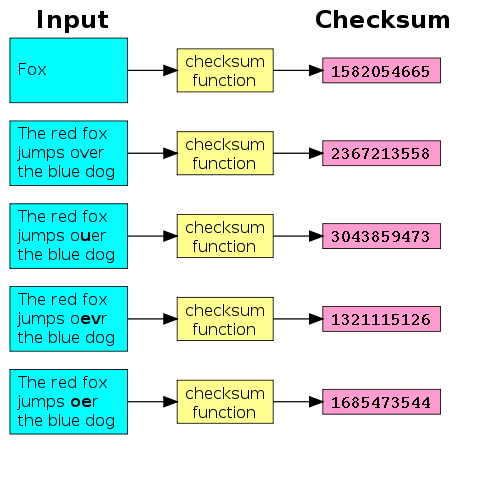
\includegraphics[scale=0.5]{checksum.png}
\end{center}
\caption{Graficna podoba kako deluje zgoščevalna funkcija}
\label{checksum_img}
\end{figure}

Te funkcije se uporabljajo tudi pri IPv4 paketih in drugje (za izračun kontrolne vsote). Funkciji podamo podatke ona pa vrne kluč oz.\ rezultat.
Pomembno je, da se zavedamo, da se pri tem izgubi informacija podatka, ki smo ga ustavili v zgoščevalno funkcijo.
Pri kriptoloških zgoščevalnih funkcijah je težko izračunati poljuben podatek, če poznamo kluč.
\\*
V UNIX operacijskih sistemih HIDS sistemi naredijo kontrolno vsoto večino datotek v /etc mapi. V /etc mapi se nahajajo konfiguracije pomembnih storitev, ki jih taka naprava/gostitelj ponuja.
Kontrolne vsote pošlje naprej nadzornemu sistemu. To naredi vsakič, ko se datoteka spremeni, ce datotečni sistem to podpira oz.\ kronološko.
\\*
Nadzorni sistem primerja prejšno vrednost z novo, če se ne ujemata uporabnika o tem obvesti.
\\*
Uporabnik nato presodi ali je to pričakovano (če je prislo do rekonfiguracije) ali pa je napadalec, ki je vdrl v sistem spremenil te datoteke.
Zato seveda uporabljano SHA1 funkcijo, ki je kriptografsko varna, kar pomeni da napadalec ne more ustvariti datoteke, ki bi imela isti kluč. Kar se pri MD5 seveda da narediti zelo poceni (oblačne storitve).
\\*

To nam pride se kako prav pri sistemih/gostiteljih, kjer posegi v konfiguracijo niso pogosti.
\\*

Eden preprostejših sistemov, ki ponuja samo to metodo zaznavanja napadov je AIDE\cite{aide}.
\\*

AIDE nam zgenerira bazo kontrolnih vsot datotek in map in jo shrani v datoteko. Nato se moramo sami potruditi in jo skopirati na drug sistem. V drugi iteraciji lahko baze med sabo primerjemo in si ogledamo rezultat sprememb.
Logiko kopiranja in primerjanja moramo napisati sami.
\\*

Imamo pa tudi bolj pametne sisteme, ki te stvari urejajo sami.
Primer sporočila, ki nam ga pošlje naprednejši sistem OSSEC iz naslova (ossecm@moon.brodul.org):

\begin{verbatim}


OSSEC HIDS Notification.
2013 Jan 11 04:44:51

Received From: moon->syscheck
Rule: 550 fired (level 7) -> "Integrity checksum changed."
Portion of the log(s):

Integrity checksum changed for: '/usr/bin/gpgsplit'
Size changed from '44664' to '44696'
Old md5sum was: 'edda24df7c85faec9d155faa7122e222'
New md5sum is : '4b47774d265adf26db424436d59501dd'
Old sha1sum was: 'e49f84977fb1c1ad10796f5071abda7b3c6810d6'
New sha1sum is : 'd80551f82582f2758cc2c22ffc15428f0399ba49'

\end{verbatim}

% paragraph Spremljanje integritete datotek (end)


\paragraph{Spremljanje dnevnikov} % (fold)

HIDS sistemi spremljajo dnevnike (logs). Tukaj ponavadi zaznajo največ poskusov napadov.
Gledajo posamezne storitve, ki so potrebne za dostop do sistema/gostitelja.
Opazujejo Telnet in ssh.
Ali so poskusi prijav skozi te sisteme uspešni ali pa niso.
Tako lahko detektirajo različne napade tako napade z pomočjo grobe sile (bruteforce) in z pomočjo slovarjev (dictionary) napade.
V kolikor se v določenem časovni periodi uporabnik prevečkrat zmoti, nas sistem o tem obvesti.
\\*

Primer sporočila, ki nam ga pošlje naprednejši sistem OSSEC iz naslova (ossecm@moon.brodul.org):

\begin{verbatim}

OSSEC HIDS Notification.
2013 Jan 10 03:24:39

Received From: moon->/var/log/auth.log
Rule: 5551 fired (level 10) -> "Multiple failed logins in a small period of time."
Portion of the log(s):

Jan 10 00:24:37 moon sshd[8999]: pam_unix(sshd:auth): authentication failure; logname= uid=0 euid=0 tty=ssh ruser= rhost=115.95.166.247  user=root
Jan 10 00:24:32 moon sshd[8997]: pam_unix(sshd:auth): authentication failure; logname= uid=0 euid=0 tty=ssh ruser= rhost=115.95.166.247  user=root
Jan 10 00:24:28 moon sshd[8995]: pam_unix(sshd:auth): authentication failure; logname= uid=0 euid=0 tty=ssh ruser= rhost=115.95.166.247  user=root
Jan 10 00:24:24 moon sshd[8993]: pam_unix(sshd:auth): authentication failure; logname= uid=0 euid=0 tty=ssh ruser= rhost=115.95.166.247  user=root
Jan 10 00:24:20 moon sshd[8991]: pam_unix(sshd:auth): authentication failure; logname= uid=0 euid=0 tty=ssh ruser= rhost=115.95.166.247  user=root
Jan 10 00:24:15 moon sshd[8989]: pam_unix(sshd:auth): authentication failure; logname= uid=0 euid=0 tty=ssh ruser= rhost=115.95.166.247  user=root
Jan 10 00:24:11 moon sshd[8987]: pam_unix(sshd:auth): authentication failure; logname= uid=0 euid=0 tty=ssh ruser= rhost=115.95.166.247  user=root
Jan 10 00:24:07 moon sshd[8985]: pam_unix(sshd:auth): authentication failure; logname= uid=0 euid=0 tty=ssh ruser= rhost=115.95.166.247  user=root



 --END OF NOTIFICATION



OSSEC HIDS Notification.
2013 Jan 10 03:24:41

Received From: moon->/var/log/auth.log
Rule: 5720 fired (level 10) -> "Multiple SSHD authentication failures."
Portion of the log(s):

Jan 10 00:24:39 moon sshd[8999]: Failed password for root from 115.95.166.247 port 35283 ssh2
Jan 10 00:24:35 moon sshd[8997]: Failed password for root from 115.95.166.247 port 34011 ssh2
Jan 10 00:24:30 moon sshd[8995]: Failed password for root from 115.95.166.247 port 60921 ssh2
Jan 10 00:24:26 moon sshd[8993]: Failed password for root from 115.95.166.247 port 59839 ssh2
Jan 10 00:24:22 moon sshd[8991]: Failed password for root from 115.95.166.247 port 58575 ssh2
Jan 10 00:24:17 moon sshd[8989]: Failed password for root from 115.95.166.247 port 57298 ssh2
Jan 10 00:24:13 moon sshd[8987]: Failed password for root from 115.95.166.247 port 56150 ssh2
Jan 10 00:24:09 moon sshd[8985]: Failed password for root from 115.95.166.247 port 54788 ssh2


 --END OF NOTIFICATION

\end{verbatim}

IP v primeru je seveda spremenjen.

% paragraph Spremljanje dnevnikov (end)

\paragraph{Zaznavanje `rootkit' zlonamernih sistemov} % (fold)

HIDS sistemi lahko detektirajo tudi takoimenovane `rootkit' sisteme.
Detekcija teh je kompleksen proces zato se v detaile nebi spuščali.

% paragraph Zaznavanje "rootkit" zlonamernih sistemov (end)

% subsubsection Nacini zaznav napadov (end)


\subsection{HIPS}

Podobno kot pri NIPS sistemih je mogoce tudi pri alarmih HIDS sistemov narediti ustrezne akcije.

\subsubsection{Načini preprečevanja napadov} % (fold)


\paragraph{Spreminjanje lokalnega požarnega zidu} % (fold)

Možno je spreminjanje pravil na lokalnem požarnem zidu (samega gostitelja).
Podobno kot pri NIPS sistemih.

\begin{verbatim}
Tue Jan  8 12:08:11 CET 2013 /opt/ossec/active-response/bin/host-deny.sh delete - h1412241.stratoserver.net 1357642659.18185 5551
Tue Jan  8 17:15:54 CET 2013 /opt/ossec/active-response/bin/firewall-drop.sh add - 198.15.109.254 1357661754.25047 5551
Tue Jan  8 17:15:54 CET 2013 /opt/ossec/active-response/bin/host-deny.sh add - 198.15.109.254 1357661754.25047 5551
Tue Jan  8 17:26:27 CET 2013 /opt/ossec/active-response/bin/host-deny.sh delete - 198.15.109.254 1357661754.25047 5551
Tue Jan  8 17:26:27 CET 2013 /opt/ossec/active-response/bin/firewall-drop.sh delete - 198.15.109.254 1357661754.25047 5551

\end{verbatim}

% paragraph Spreminjanje lokalnega pozarnega zidu (end)

\paragraph{Suspendacija uporabnika za določen čas} % (fold)

Ponavadi HIPS sistemi omogočajo izklop avtentikacije za določega uporabnika na samem sistemu.
Torej izklopijo uporabnika za časovno obdobje napada, nato pa ga spet vklopijo.

% paragraph Suspendacija uporabnika za dolocen cas (end)

\paragraph{Povrnitev nastavitev} % (fold)

Če se zazna sprememba konfiguracije, je mogoče ob spremembi skopirati konfiguracijske datoteke iz oddaljenega sistema.

% paragraph Povrnitev nastavitev (end)

\paragraph{Odjava napadalca} % (fold)

Če je uporabnik neavtorizirano prijavljen, ga lahko odjavimo od seje.

% paragraph Odjava napadalca (end)


% subsubsection Nacini preprecevanja napadov (end)


\section{Praktični del}

\subsection{Nameščanje programske opreme Snort}
\subsection{Zmožnosti Snort programja}
\subsection{Spletni vmesnik za Snort}
\subsection{Praktični primeri napadov}

\section{Rezultati}

Bla bla.

\clearpage
\addcontentsline{toc}{section}{Viri}
\begin{thebibliography}{9}


\bibitem{eaptypes}
Snort Manual, \url{http://manual.snort.org/}, 20.12.2012

\bibitem{cisco5000}
Cisco ASA 5000 serije, \url{http://www.cisco.com/en/US/products/ps6120/prod_models_comparison.html}, 27.12.2012

\bibitem{aide}
AIDE, \url{http://aide.sourceforge.net/}, 27.12.2012

\bibitem{sourcefire}
SourceFire, \url{http://en.wikipedia.org/wiki/Sourcefire,_Inc}, 27.12.2012

\bibitem{snort}
Snort, \url{http://www.snort.org/}, 27.12.2012

\bibitem{oisf}
OISF, \url{https://www.openinfosecfoundation.org/}, 27.12.2012

\bibitem{komponente}
Slika \ref{komponente}, 
Narisal Andraž Brodnik, 29.12.2012

\bibitem{pozicija}
Slika \ref{pozicija}, 
Narisal Andraž Brodnik, 29.12.2012

\bibitem{snort_img}
Slika \ref{snort_img}, 
\url{http://en.wikipedia.org/wiki/File:Snort_ids_logo.png}, 29.12.2012

\bibitem{cisco_img}
Slika \ref{cisco_img}, 
\url{http://en.wikipedia.org/wiki/File:Cisco_logo.svg}, 29.12.2012

\bibitem{checksum_img}
 Slika \ref{checksum_img}, 
\url{http://en.wikipedia.org/wiki/File:Checksum.svg}, 29.12.2012

\end{thebibliography}
\end{document}



